% Preambulo compartido para clases en formato beamer
\documentclass[9pt, xcolor=svgnames]{beamer}
\usepackage[utf8]{inputenc}
\usepackage[T1]{fontenc}
\usepackage[spanish,es-nodecimaldot]{babel}

\usetheme[progressbar=frametitle]{metropolis}
\metroset{sectionpage=none, subsectionpage=none}
\usepackage{appendixnumberbeamer}
\usepackage{booktabs}
\usepackage{amsmath,amssymb,bm,mathtools}
\usepackage{physics}
\usepackage{graphicx}
\usepackage{multicol}
\usepackage{tikz}
\usepackage{minted}
\usemintedstyle{tango}
\setminted{fontsize=\scriptsize, breaklines=true, linenos=true, bgcolor=LightGray!20, frame=lines}
\newminted{python}{fontsize=\scriptsize, breaklines=true, linenos=true, bgcolor=LightGray!20, frame=lines}
\usepackage{pgfplots}
\pgfplotsset{compat=1.18}
\usepackage{ragged2e}
\usepackage{xspace}
\newcommand{\themename}{\textbf{\textsc{metropolis}}\xspace}

\setbeamercolor{block title}{bg=MidnightBlue!85, fg=white}
\setbeamercolor{block body}{bg=MidnightBlue!5, fg=black}
\setbeamercolor{alerted text}{fg=Crimson}
\setbeamercolor{frametitle}{bg=MidnightBlue!10, fg=black}
\setbeamertemplate{blocks}[rounded][shadow=true]


% Curso: Modelos Computacionales PCFI261 - Semana 05
% Tema: Metodos de simulacion Monte Carlo

\weektitle{05}{Métodos de Simulación Monte Carlo}

\begin{document}

\frame{\titlepage}

\begin{frame}{Organización de la semana}
\small
\begin{block}{Formato de las clases}
Las sesiones se dividen en dos clases, manteniendo el formato de semanas anteriores:
\begin{itemize}
    \item \textbf{30--45 min} de teoría y discusión conceptual.
    \item \textbf{75--90 min} de laboratorio guiado con Python.
\end{itemize}
\end{block}

\vspace{0.15cm}
\begin{columns}[T,onlytextwidth]
\column{0.48\textwidth}
\textbf{Clase 1}
\begin{itemize}
    \setlength\itemsep{0.2em}
    \item Fundamentos de Monte Carlo.
    \item Ley de los grandes números.
    \item Números pseudoaleatorios.
    \item Estimación de $\pi$ por muestreo.
    \item Caminata al azar en una dimensión.
\end{itemize}

\column{0.48\textwidth}
\textbf{Clase 2}
\begin{itemize}
    \setlength\itemsep{0.2em}
    \item Distribución normal y TCL.
    \item Variables gaussianas en Python.
    \item Método del rechazo.
    \item Movimiento browniano.
    \item Actividades y ejercicios.
\end{itemize}
\end{columns}
\end{frame}

\section{Clase 1}

\begin{frame}[plain]
\centering
\vfill
{\Huge \bfseries Clase 1}\\[0.4cm]
{\Large Fundamentos de los métodos Monte Carlo}
\vfill
\end{frame}

\begin{frame}{Objetivos de la Clase 1}
Al terminar esta clase, usted será capaz de:
\begin{itemize}
    \item Entender cómo los métodos de Monte Carlo convierten integrales en promedios de variables aleatorias.
    \item Describir la ley de los grandes números y su rol en la estimación de expectativas.
    \item Implementar generadores de números pseudoaleatorios simples y utilizar los suministrados por Python.
    \item Aplicar Monte Carlo para estimar el área de un círculo y aproximar $\pi$.
    \item Simular una caminata al azar en una dimensión y analizar su comportamiento.
\end{itemize}
\end{frame}

\begin{frame}{¿Qué son los métodos de Monte Carlo?}
\justifying
Los métodos de Monte Carlo engloban un conjunto de algoritmos que utilizan
\emph{ensayos aleatorios} para aproximar cantidades deterministas. Su uso es
particularmente valioso cuando se trata de calcular promedios o integrales en
altas dimensiones, donde los métodos deterministas se vuelven prohibitivos.

De forma general, si queremos evaluar
\begin{equation*}
I = \int_{\Omega} f(\bm{x})\, d\bm{x},
\end{equation*}
podemos elegir muchos puntos aleatorios $\bm{x}_1,\dots,\bm{x}_N$ dentro de la
región $\Omega$.

\begin{block}{¿Qué es un estimador?}
Un \textbf{estimador} es una fórmula que, usando una muestra finita de datos,
nos entrega una \textbf{aproximación} de una cantidad desconocida. En este
caso, queremos aproximar la integral $I$.
\end{block}

\begin{itemize}
    \item Cada punto aleatorio nos da un valor de la función: $f(\bm{x}_i)$.
    \item Si promediamos muchos de esos valores, obtenemos una idea del valor típico de $f$ en la región.
    \item Luego ese promedio se ajusta por el tamaño de la región para aproximar la integral.
\end{itemize}
\end{frame}

\begin{frame}{La fórmula del estimador Monte Carlo}
\justifying
Si el volumen de la región es
\begin{equation*}
V = \int_{\Omega} d\bm{x},
\end{equation*}
entonces el estimador Monte Carlo de la integral es
\begin{equation*}
Q_N = V\,\frac{1}{N}\sum_{i=1}^N f(\bm{x}_i).
\end{equation*}
\begin{block}{Cómo leer esta fórmula}
\begin{itemize}
    \item $\frac{1}{N}\sum_{i=1}^N f(\bm{x}_i)$ es el promedio de los valores de la función.
    \item $V$ corrige ese promedio por el tamaño total de la región.
    \item $Q_N$ es, entonces, nuestra \textbf{mejor aproximación numérica} de la integral usando $N$ puntos.
\end{itemize}
\end{block}

\begin{alertblock}{Idea intuitiva}
Integrar es sumar contribuciones en toda una región. Monte Carlo reemplaza esa
suma exacta por un \textbf{promedio aleatorio} multiplicado por el volumen.
\end{alertblock}
\end{frame}

\begin{frame}{Ejemplo simple: $f(x)=x^2$ en $[0,1]$}
\justifying
Supongamos que queremos calcular
\begin{equation*}
I=\int_0^1 x^2\,dx.
\end{equation*}
Sabemos por cálculo que el valor exacto es
\begin{equation*}
I=\frac{1}{3}\approx 0.333.
\end{equation*}

\begin{block}{¿Cuál es el ``volumen'' aquí?}
En una dimensión, el volumen de la región es simplemente la longitud del
intervalo:
\begin{equation*}
V=\int_\Omega dx=\int_0^1 dx=1.
\end{equation*}
\end{block}

Así, en este caso el estimador Monte Carlo queda especialmente simple:
\begin{equation*}
Q_N = \frac{1}{N}\sum_{i=1}^N x_i^2.
\end{equation*}
\end{frame}

\begin{frame}{Calculando $Q_N$ con numeritos}
\justifying
Imaginemos que el azar nos dio estos cuatro puntos:
\begin{equation*}
x_1=0.2,\qquad x_2=0.5,\qquad x_3=0.8,\qquad x_4=0.9.
\end{equation*}

Entonces
\begin{equation*}
f(x_1)=0.04,\quad f(x_2)=0.25,\quad f(x_3)=0.64,\quad f(x_4)=0.81.
\end{equation*}

El promedio es
\begin{equation*}
\frac{0.04+0.25+0.64+0.81}{4}=\frac{1.74}{4}=0.435.
\end{equation*}

Como aquí $V=1$, obtenemos
\begin{equation*}
Q_4 = 1\times 0.435 = 0.435.
\end{equation*}

\begin{alertblock}{Interpretación}
No coincide exactamente con $1/3$ porque usamos muy pocos puntos. Si tomamos
muchos más, $Q_N$ debería acercarse al valor verdadero de la integral.
\end{alertblock}
\end{frame}

\begin{frame}[fragile]{Python: estimando $\int_0^1 x^2\,dx$ con Monte Carlo}
\inputminted[fontsize=\scriptsize]{python}{montecarlo_x2.py}
\end{frame}

\begin{frame}{Qué queremos que se vea en este ejemplo}
\begin{itemize}
    \item La integral exacta existe y vale $1/3$.
    \item Monte Carlo no ``adivina'' ese valor: lo aproxima usando promedios.
    \item El factor $V$ representa el tamaño de la región donde estamos muestreando.
    \item En $[0,1]$, como $V=1$, la fórmula se simplifica mucho.
    \item En regiones más grandes o en más dimensiones, la idea es la misma.
\end{itemize}
\end{frame}

\begin{frame}{Ley de los grandes números}
\justifying
La \textbf{ley de los grandes números} explica por qué Monte Carlo funciona.
Si evaluamos una variable aleatoria $Y=f(\bm{X})$ muchas veces de manera
independiente, entonces su promedio muestral
\begin{equation*}
\overline{Y}_N = \frac{1}{N}\sum_{i=1}^{N} Y_i
\end{equation*}
se acerca al valor esperado $\mathbb{E}[Y]$ cuando $N$ crece.

\begin{itemize}
    \item No garantiza que cada muestra individual sea buena.
    \item Sí garantiza que el \textbf{promedio} de muchas muestras se estabiliza.
    \item Esa es la idea central detrás de cualquier estimación Monte Carlo.
\end{itemize}

\begin{alertblock}{Interpretación física y numérica}
Si una magnitud difícil de calcular puede escribirse como un valor esperado,
entonces podemos aproximarla generando muchas realizaciones aleatorias y
promediándolas.
\end{alertblock}
\end{frame}

\begin{frame}{¿Dónde aparece $Q_N$ en Monte Carlo?}
\small
\justifying
En integración Monte Carlo, tomamos puntos aleatorios $\bm{x}_i$ en la región
$\Omega$ y construimos el estimador
\begin{equation*}
Q_N = V\,\frac{1}{N}\sum_{i=1}^{N} f(\bm{x}_i),
\end{equation*}
que aproxima la integral
\begin{equation*}
I = \int_{\Omega} f(\bm{x})\,d\bm{x}.
\end{equation*}

\begin{block}{Idea clave}
$Q_N$ no es una letra más: es la \textbf{respuesta numérica} que entrega el
algoritmo. Cuando $N$ aumenta, esperamos que $Q_N$ se acerque cada vez más al
valor verdadero $I$.
\end{block}

\begin{itemize}
    \setlength\itemsep{0.2em}
    \item Si aumentamos $N$, el promedio se estabiliza.
    \item El error típico baja como $N^{-1/2}$, por lo que reducirlo mucho requiere más muestras.
    \item La gracia de Monte Carlo es transformar una integral difícil en un promedio fácil de simular.
\end{itemize}
\end{frame}

\begin{frame}{Generación de números pseudoaleatorios}
\justifying
Para implementar simulaciones Monte Carlo necesitamos secuencias de números
\emph{pseudoaleatorios}. Un generador muy usado en ejemplos pedagógicos es el
\textbf{generador lineal congruente (GLC)}, definido por
\begin{equation*}
X_{n+1} = (A\,X_n + C) \bmod m.
\end{equation*}
Al elegir adecuadamente las constantes $A$, $C$ y $m$, la secuencia resultante
recorre un periodo largo antes de repetirse. Un ejemplo clásico utiliza
$A=1664525$, $C=1013904223$ y $m=2^{32}$.

Aun siendo sencillo, este método no es adecuado para aplicaciones sensibles.
Por ello, en la práctica utilizamos librerías de calidad como \texttt{random}
o \texttt{numpy.random} en Python. A continuación se ilustra cómo generar
números uniformes y cómo producir eventos con probabilidad $p$.

\begin{block}{Generar un evento con probabilidad $p$}
\begin{enumerate}
    \item Genere un número $r$ uniforme en el intervalo $[0,1]$.
    \item Si $r<p$, entonces el evento ocurre; en caso contrario, no ocurre.
\end{enumerate}
\end{block}
\end{frame}

\begin{frame}{Estimación del área de un círculo}
\normalsize
\justifying
Considere el problema de calcular el área de un círculo de radio $R$ mediante
Monte Carlo. El área exacta es $\pi R^2$, pero podemos estimarla muestreando
puntos uniformes en un cuadrado que circunscribe al círculo. Sea
$\Omega=[-R,R]\times[-R,R]$ de área $V=(2R)^2$ y definamos la función
indicadora
\begin{equation*}
H(x,y)=
\begin{cases}
1 & \text{si } x^2+y^2 \le R^2,\\
0 & \text{en otro caso.}
\end{cases}
\end{equation*}
\end{frame}

\begin{frame}{Estimación de $\pi$ con Monte Carlo}
\normalsize
\justifying
La integral que da el área es $I=\int_{\Omega} H(x,y)\,dx\,dy$, de modo que
$I/V=\langle H\rangle$. Así, la estimación se construye como
\begin{equation*}
Q_N = V\,\frac{1}{N}\sum_{i=1}^N H(x_i,y_i),
\end{equation*}
con $(x_i,y_i)$ generados uniformemente en $\Omega$. El valor $Q_N/V$ tiende a
$\pi$ cuando $N$ es grande.
\end{frame}

\begin{frame}[fragile]{Código: estimación de $\pi$ por Monte Carlo}
\begin{columns}[T,onlytextwidth]
\column{0.5\textwidth}
\inputminted[firstline=6,lastline=18,fontsize=\scriptsize]{python}{circle.py}

\column{0.45\textwidth}
\small
\begin{block}{Qué está pasando}
\begin{itemize}
    \item Se generan puntos al azar en un cuadrado.
    \item Se revisa cuáles caen dentro del círculo.
    \item Contar ``aciertos'' permite estimar el área.
\end{itemize}
\end{block}
\end{columns}
\end{frame}

\begin{frame}[fragile]{Resultado visual de la simulación}
\begin{columns}[T,onlytextwidth]
\column{0.45\textwidth}
\inputminted[firstline=20,lastline=24,fontsize=\tiny]{python}{circle.py}

\column{0.55\textwidth}
\begin{center}
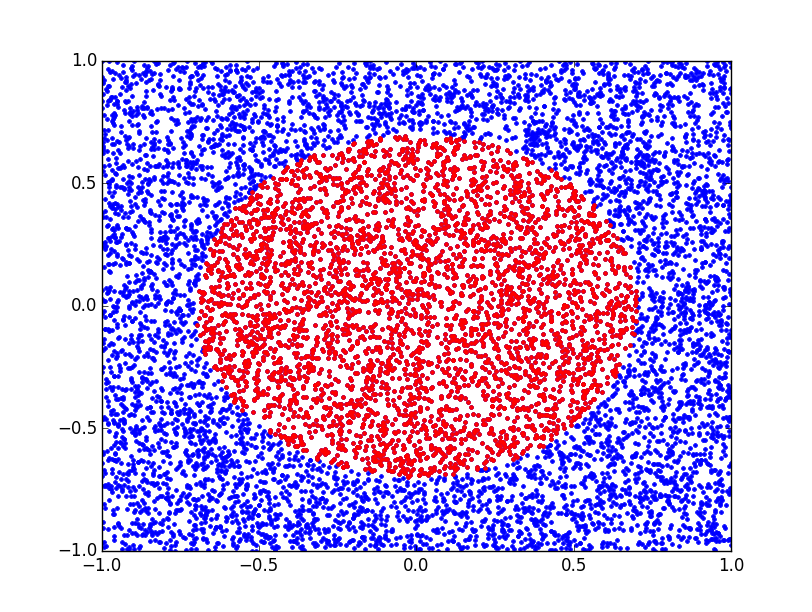
\includegraphics[width=\linewidth]{circle.png}
\end{center}
\small
Azul: puntos en el cuadrado. Rojo: puntos dentro del círculo. La fracción de
puntos rojos aproxima la razón de áreas y, con ella, el valor de $\pi$.
\end{columns}
\end{frame}

\begin{frame}{Caminata al azar en una dimensión}
\justifying
Otra aplicación básica de Monte Carlo es la \textbf{caminata al azar} en una
dimensión. El algoritmo puede escribirse de la siguiente manera:
\begin{enumerate}
    \item Inicialice la posición en $x_0=0$.
    \item Repita $n$ veces: con probabilidad $p$ avance una distancia $\Delta x$
          al azar en $[0,1]$; con probabilidad $1-p$ retroceda una distancia
          $\Delta x$ en $[0,1]$.
    \item Registre la posición $x_n$ y analice su distribución.
\end{enumerate}
Gracias al teorema central del límite, la distribución de $x_n$ tiende a ser
gaussiana para pasos grandes y varianza proporcional a $n$.
\end{frame}

\begin{frame}{Resumen de la Clase 1}
\begin{itemize}
    \item Convertir integrales en promedios es la esencia de los métodos de Monte Carlo.
    \item La ley de los grandes números garantiza convergencia y un error decreciente como $N^{-1/2}$.
    \item Los generadores pseudoaleatorios permiten crear secuencias reproducibles y uniformes; los lenguajes modernos incluyen implementaciones robustas.
    \item La estimación de $\pi$ mediante puntos al azar ilustra cómo se transforman problemas geométricos en conteo de éxitos.
    \item Las caminatas al azar son un puente hacia procesos continuos como el movimiento browniano.
\end{itemize}
\end{frame}

\section{Clase 2}

\begin{frame}[plain]
\centering
\vfill
{\Huge \bfseries Clase 2}\\[0.4cm]
{\Large Muestreo avanzado y movimiento browniano}
\vfill
\end{frame}

\begin{frame}{Objetivos de la Clase 2}
Al completar esta clase, usted podrá:
\begin{itemize}
    \item Reconocer la importancia de la distribución normal y su relación con el teorema central del límite.
    \item Generar variables gaussianas a partir de funciones de Python y comparar con su densidad teórica.
    \item Implementar el método del rechazo para muestrear distribuciones arbitrarias.
    \item Modelar trayectorias de movimiento browniano en dos dimensiones y calcular el desplazamiento cuadrático medio.
\end{itemize}
\end{frame}

\begin{frame}{La distribución normal o gaussiana}
\small
\justifying
La distribución normal, también llamada gaussiana, es quizá la distribución
continua más importante en estadística y física. Su función de densidad de
probabilidad general está dada por
\begin{equation*}
f(x) = \frac{1}{\sqrt{2\pi\,\sigma^{2}}}\,\exp\Bigl[-\tfrac{1}{2}\bigl(\tfrac{x-\mu}{\sigma}\bigr)^2\Bigr],
\end{equation*}
donde $\mu$ es el valor esperado y $\sigma^2$ la varianza de la distribución.
La normalidad surge de manera natural gracias al teorema central del límite:
la media de muchas variables independientes y de varianza finita converge a una
normal.

\vspace{0.3cm}
\begin{center}
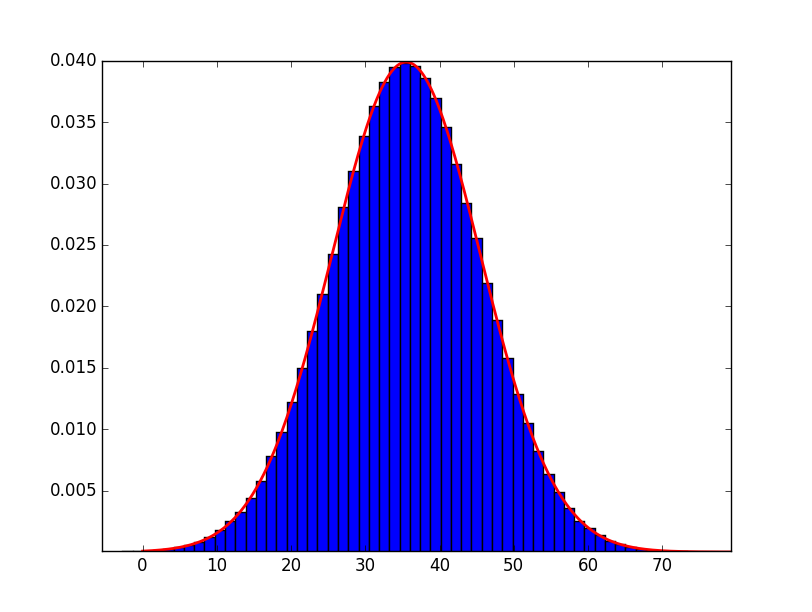
\includegraphics[width=0.48\textwidth]{gaussian.png}
\end{center}
\end{frame}

\begin{frame}[fragile]{Generación de variables gaussianas}
\small
\justifying
Existen varios algoritmos para generar muestras con distribución normal. Python
ofrece funciones ya implementadas (\texttt{random.gauss()} o
\texttt{numpy.random.normal()}) basadas en transformaciones como Box--Muller.
El siguiente código genera $10^5$ muestras con media $\mu=2$ y desviación
estándar $\sigma=1.5$, construye un histograma normalizado y lo compara con
la densidad teórica:

\inputminted[fontsize=\tiny]{python}{gaussianhistogram.py}
\end{frame}

\begin{frame}{Método del rechazo}
\small
\begin{columns}[T,onlytextwidth]
\column{0.55\textwidth}
\justifying
Cuando deseamos muestrear de una distribución $p(x)$ que no tiene una fórmula
inversa simple, podemos utilizar el \textbf{método del rechazo}. Este método
requiere una función auxiliar $g(x)$ fácilmente muestreable y una constante $c$
tal que $p(x)\le c\,g(x)$ para todo $x$.
\begin{enumerate}
    \item Muestre un valor $x$ de la distribución $g(x)$.
    \item Genere un número $r$ uniforme en $[0,1]$.
    \item Acepte $x$ si $r < p(x)/(c\,g(x))$.
    \item Si no se acepta, repita el proceso.
\end{enumerate}
El ratio de aceptación depende de la calidad de la cota $c$.

\column{0.45\textwidth}
\begin{center}
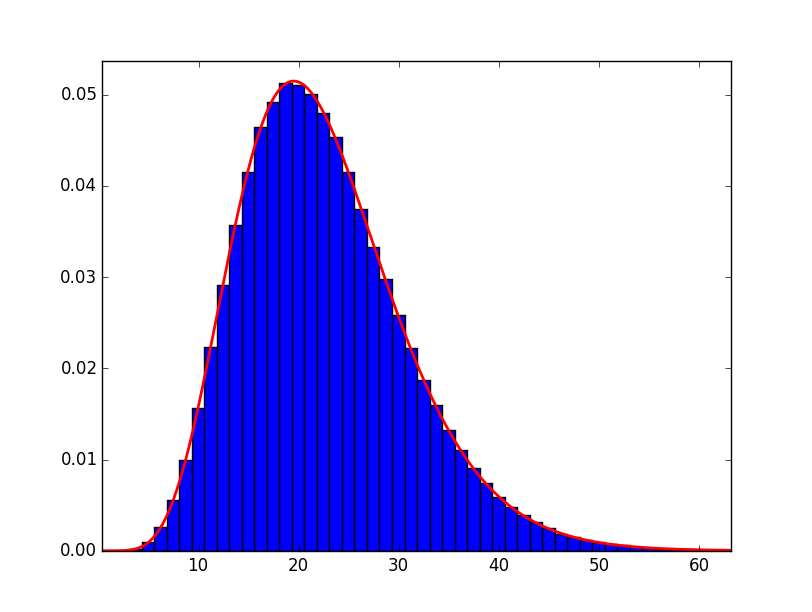
\includegraphics[width=\linewidth]{rejection.png}
\end{center}
\end{columns}
\end{frame}

\begin{frame}{Movimiento browniano}
\small
\justifying
El \textbf{movimiento browniano} describe la trayectoria errática de una
partícula en un fluido y es modelado matemáticamente por el proceso de Wiener
$W_t$. Se caracteriza por cuatro propiedades:
\begin{itemize}
    \item $W_0 = 0$.
    \item Las trayectorias son continuas casi seguramente.
    \item Los incrementos son independientes: $W_{t_2}-W_{s_2}$ es independiente de $W_{t_1}-W_{s_1}$ para intervalos no solapados.
    \item Los incrementos tienen distribución normal: $W_t-W_s \sim \mathcal{N}(0,t-s)$.
\end{itemize}
En una simulación discreta tomamos pasos $\Delta t$ pequeños y generamos
incrementos $\Delta x,\Delta y \sim \mathcal{N}(0,\sigma^2\,\Delta t)$,
acumulándolos para obtener la trayectoria. El desplazamiento cuadrático medio
obedece $\langle|\bm{r}(t)-\bm{r}(0)|^2\rangle = 2d\sigma^2 t$, donde $d$ es la
dimensión.
\end{frame}

\begin{frame}{Actividades de la semana}
\small
\begin{enumerate}
    \setlength\itemsep{0.35em}
    \item \textbf{Random walk:} Escriba un programa que simule una caminata al azar en una dimensión con probabilidad $p=0.6$ de ir a la derecha y $1-p=0.4$ de ir a la izquierda. El paso $\Delta x$ debe ser un número uniforme en $[0,1]$. Grafique la distribución de posiciones luego de 15 y 30 pasos para $50\,000$ realizaciones.
    \item \textbf{Muestreo gaussiano:} Utilice el método del rechazo para generar un millón de números con distribución gaussiana de media $\mu=2$ y varianza $\sigma^2=1.5$. Compare el histograma con muestras generadas por \texttt{numpy.random.normal}.
    \item \textbf{Movimiento browniano:} Simule trayectorias brownianas en dos dimensiones con $\sigma=1$ para $t=100$, $500$, $1000$, $5000$ y $10\,000$ pasos. Para cada $t$ promedie $\langle|\bm{r}(t)|^2\rangle$ sobre 10, 100 y 500 realizaciones y discuta la dependencia temporal.
    \item \textbf{Estimación de $\pi$ adicional:} Modifique el ejemplo de la estimación del área de un círculo para calcular $\pi$ en dimensión tres, contando la proporción de puntos dentro de una esfera de radio unidad dentro de un cubo circunscrito.
\end{enumerate}
\end{frame}

\begin{frame}{Resumen de la Clase 2}
\begin{itemize}
    \item La distribución normal describe muchos fenómenos naturales y su densidad está determinada por sus dos parámetros, media y varianza.
    \item Python facilita generar variables gaussianas y comparar con la curva teórica para verificar la calidad del muestreo.
    \item El método del rechazo permite muestrear distribuciones complejas a expensas de rechazar algunos puntos; la eficiencia mejora con cotas ajustadas.
    \item El movimiento browniano es un proceso con incrementos normales e independientes; su simulación discreta es una generalización de la caminata al azar.
    \item Las actividades propuestas consolidan la teoría mediante programación y análisis numérico.
\end{itemize}
\end{frame}

\end{document}
